%------------------------------------------------------------------------
%  交通流のシミュレーション 
%  The Mathematical Society of Traffic Flow
%  
%  Ver. 1.0 05/12/09  H. Watanabe
%------------------------------------------------------------------------

%\documentclass[twocolumn]{jarticle} %二段組の場合
\documentclass[twocolumn,dvipdfmx]{jarticle}
%\documentclass[dvipdfmx]{article}
%\documentclass[onecolumn]{jarticle}  %一段組の場合

\usepackage{mstf2}

\usepackage{color}
\usepackage[dvipdfmx]{graphicx}
\usepackage{comment}

%\usepackage[dviout]{graphicx}

%\graphicspath{{../pic/}}
%------------------------------------------------------------------------

\title{%和文タイトル
最適速度旋回アルゴリズムによるスキッドステアリング\\
2Dロボットのひも状走行
}

\titleE{%英文タイトル
String-like traveling of skid-steering 2D robots by Optimal Verocity Turning Algorithm
}

\author{%和文氏名
山田 将司$^1$,李 方正$^1$,本田 泰$^2$
}

\authorE{%英文氏名
Masashi Yamada$^1$,Li Fangzheng$^1$, Yasushi Honda$^2$
}

\affiliation{%和文所属
$^1$ 室蘭工業大学大学院 工学研究科 情報電子工学系専攻\\
$^2$ 室蘭工業大学大学院 しくみ解明系領域
}

\affiliationE{%英文所属
$^1$ Division of Information and Electronic Engineering, Graduate school of Engineering, Muroran Instutude of Technology, Japan \\
$^2$ College of Information and System, Muroran Institude of Technology, Japan
}

\abst{%和文概要
我々は以前,二次元最適速度モデルという自己駆動モデルを知能として組み込んだ2次元最適速度ロボットを開発した.
今回新たに,スキッドステアリングにより4輪で走行するロボットを開発した.
以前の2輪走行アルゴリズムをもとに,スキッドステアによる4輪走行のための2次元最適速度旋回アルゴリズムを導出した.
また,接触センサから距離センサに変更することで,障害物に衝突する前に方向転換を行うようにアルゴリズムを変更した.
本研究の目的は2輪の走行ロボットで観測されたひも状走行が4輪のロボットでも観測できるか実験を行った.
結果として,4輪の走行ロボットでもひも状走行は観測された.

}

\abstE{%英文概要
We have developed the 2D optimal velocity robot which is made by incorporating a self-driven model which is named the 2D optimal velocity model previously.
And recently, we also developed a robot that run by four whells with skid steering.
Then, we derived a 2D optimal velocity turning algorithm for four-wheels driving by skid steering based on the two-wheel driving algorithm previously.
In addition, by changing from the contact sensor to the distance sensor, the algorithm also is changed to another algorithm which operates as robot's direction change before colliding with obstacles.
The purpose of this study was to check if the string-like motion can be observed by the four-wheels land-moving robot as same as two-wheels land-moving robot.
As a result, string-like motion was also observed with a four-wheel land-moving robots.
}

%------------------------------------------------------------------------
% ここから本文
%------------------------------------------------------------------------

\begin{document}
\maketitle
\section{はじめに}
\vspace{-2mm}
歩行者や交通渋滞といった集団行動は,各個体の相互作用によって自己組織的に形成される動きである.
我々はその中で交通流モデルである一次元最適速度モデルを2次元に拡張した2次元最適速度ロボットを開発した\cite{mygm}.

環境と走行ロボットが相互作用することで行動を創発する.
本研究では,スキッドステアリングで走行するロボットを使用して実験を行った.
スキッドステアリングとは,スキッド(滑る)とステアリング(操舵)という駆動方法であり,タイヤを滑らせながら走行する駆動方法である.
走行ロボットの身体性が変化しても,先行研究\cite{mygm}と同じひも状走行が観測されるか確かめることを本研究の目的とする.

%身体性の変更により,走行アルゴリズムを新たに導出し,そのアルゴリズムを用いたロボットを使って実験を行うことで,集団行動が見られるかを調べた.
\vspace{-4mm}
\section{2次元最適速度モデル}
2次元最適速度モデルは以下の運動方程式(\ref{model_1})式で表される\cite{ov2}.
自己のロボットの速度と最適速度の差から,加速度を求めるモデルである.
\begin{eqnarray}
\label{model_1}
{\bf \ddot{r}}_{j} = a\left[ \sum_{k} {\bf V} \left({\bf r}_{kj},{\bf \dot{r}}_{j}\right) - {\bf \dot{r}}_{j} \right] \\
\label{model_2}
{\bf V}({\bf {r}}_{kj} , {\bf \dot{r}}_j) = (1+\cos\theta_{kj}) f\left(r_{kj}\right)  \mbox{\boldmath $n$}_{kj} \\
f(r_{kj}) = \alpha  \left[ \tanh\beta(r_{kj} - b ) + c \right]
\label{model_3}
\vspace{-2mm}
\end{eqnarray}

$ {\bf V}({\bf r}_{kj},{\bf \dot{r}}_{j}) $は$j$番目のロボットが$k$番目のロボットから受ける相互作用項である.
$\mbox{\boldmath $n$}_{kj}$は${\bf r}_{kj}$の単位ベクトルを表す.
$\theta_{kj}$は$j$番目のロボットの速度ベクトル${\bf \dot{x}}_j$と相対位置${\bf r}_{kj}$のなす角であり(\ref{model_2})式で与えられる.$(1+\cos\theta_{kj})$は異方性を表す項である.
モデル上では,$\mbox{\boldmath $n$}_{kj}$は${\bf r}_{kj}$の単位ベクトルだが,ロボットに組み込む際に,$\mbox{\boldmath $n$}_{kj} = (\sin(\theta_{kj}),\cos(\theta_{kj}))$と近似した.
$f(r_{kj})$は最適速度関数(\ref{model_3})式であり,ロボットとの距離$r_{kj}$に応じて引力または斥力を決定する関数である.

本研究ではこのモデルを離散化し,走行ロボットの速度ベクトルを走行ロボットの前進する速度と旋回する速度に変換する必要がある.
$\Delta t$秒後の${\bf \dot{r}}_j$を離散化して求めると(\ref{model_4})式となる.
(\ref{model_2})式中の$\theta_{kj}$は$360^{\circ}$反応できる範囲があるが,ロボットに搭載されているカメラの画角は約$104^{\circ}$である.
よって,$ -52^{\circ}< \theta_{kj} < 52^{\circ}$でなければ,カメラで他機体を認識できない.

4輪の接地面での速度$v_L$,$v_R$を(\ref{left})(\ref{right})式で求める.
ここでの$v_L$は進行方向左側の車輪の速度,同様に$v_R$は右の車輪の速度を表す.

先行研究\cite{mygm}では角加速度を用いて計算していたが,本研究では角速度$\omega$を用いることとした.
角加速度を用いて計算した場合,走行ロボットはスキッドステアで旋回するため,本来の旋回角度と実際にロボットが旋回した角度にズレが生じてしまうためである.
また,$d$は車輪とロボットの中心からの距離で本来であれば0.13[m]だが本研究では$d$を旋回力を調整するゲインとして扱うことにし,$d=5$[m]とした.
旋回方法の変更により,(\ref{left})式,(\ref{right})式内部の$d$は車輪とロボット中心間の距離としていたが,$d$を実際の値よりも大きくすることでより強い旋回力を得られるように変更した.
$d$はロボットの半径を意味する値である.
本来であれば,$d=0.07$であるが,本研究で使用するロボットはスキッドステアで走行するため,先行研究\cite{yamada}のロボットと比べてより多くの旋回力が必要である.
本研究では$d=5.0$設定し,$d$を調整可能なパラメータとして扱うこととした.

%$d$の値はロボットの中心からの距離の0.07[m]に設定して実験を行っていたが,ロボットの動きを目視で確認し,旋回力が弱いと判断したため,$d=1.0$[m]に変更した.
%それでも旋回力が弱かったため,$d=5.0$[m]と設定した.本研究では$d=5.0$[m]で実験を行った場合の結果である.

\vspace{-2.5mm}
\begin{eqnarray}
\label{model_4}
{\bf \dot{r}}_j(t+\Delta t) = {\bf \dot{r}}_j(t) + \Delta t {\bf \ddot{r}}_j (t) \\
\label{model_6}
{\bf \dot{r}}_j(t+\Delta t) = (\dot{x}_{j}(t+\Delta t) , \dot{y}_{j}(t+\Delta t))\\
\label{model_omega}
\omega = \arctan(\frac{\dot{x}_{j}(t+\Delta t)}{\dot{y}_{j}(t+\Delta t)}) \\
\label{left}
v_L(t + \Delta t) = \dot{r}_j(t + \Delta t) + d \cdot \omega\\
\label{right}
v_R(t + \Delta t) = \dot{r}_j(t + \Delta t) - d \cdot \omega
\end{eqnarray}
%\vspace{-17mm}
\section{2次元最適速度ロボットの身体性}
本研究では4輪駆動の走行ロボット図(\ref{fig:ssr1}),(\ref{fig:ssr2})で実験を行う.
先行研究\cite{mygm}では2輪とボールキャスターの走行ロボットであったが,本研究ではスキッドステアリングにより4輪で走行するロボットを使用する.
本研究では,4輪の走行ロボットを使用し,図\ref{fig:ssr2}中央のギヤを回転させることで,左右それぞれのタイヤに駆動力を伝達するスキッドステアリングで方向転換を行う.2輪から4輪へと変更した理由としては,2輪とボールキャスターでは地面に段差や凹凸があるとうまく走行できない.
4輪の場合だと走破性が高く,段差や凹凸があっても2輪走行と比べ,比較的安定して走行が可能である.

本研究で使用するロボットにはtofセンサとカメラ,2つのモータを用いる.
カメラはRaspberry Pi Cameraというカメラで,他のロボットの方角と距離を検出している.
tof距離センサでは走行ロボットと壁や他機体との距離を測定している.
進行方向前方にtofセンサーを3つ装着している.中央に装着しているtof距離センサは進行方向正面向きに装着,左右のtof距離センサは進行方向正面から左右$45^{\circ}$外側に向けて装着している.
2種類のセンサから得られた情報を利用して走行ロボットは2つのサーボモーターを動かし移動する.
\newpage
\vspace{-2cm}
\begin{figure}[h]
\begin{center}
  %\includegraphics[width=0.8\linewidth,height=6.0cm]{pic/DSC_5332.JPG}
  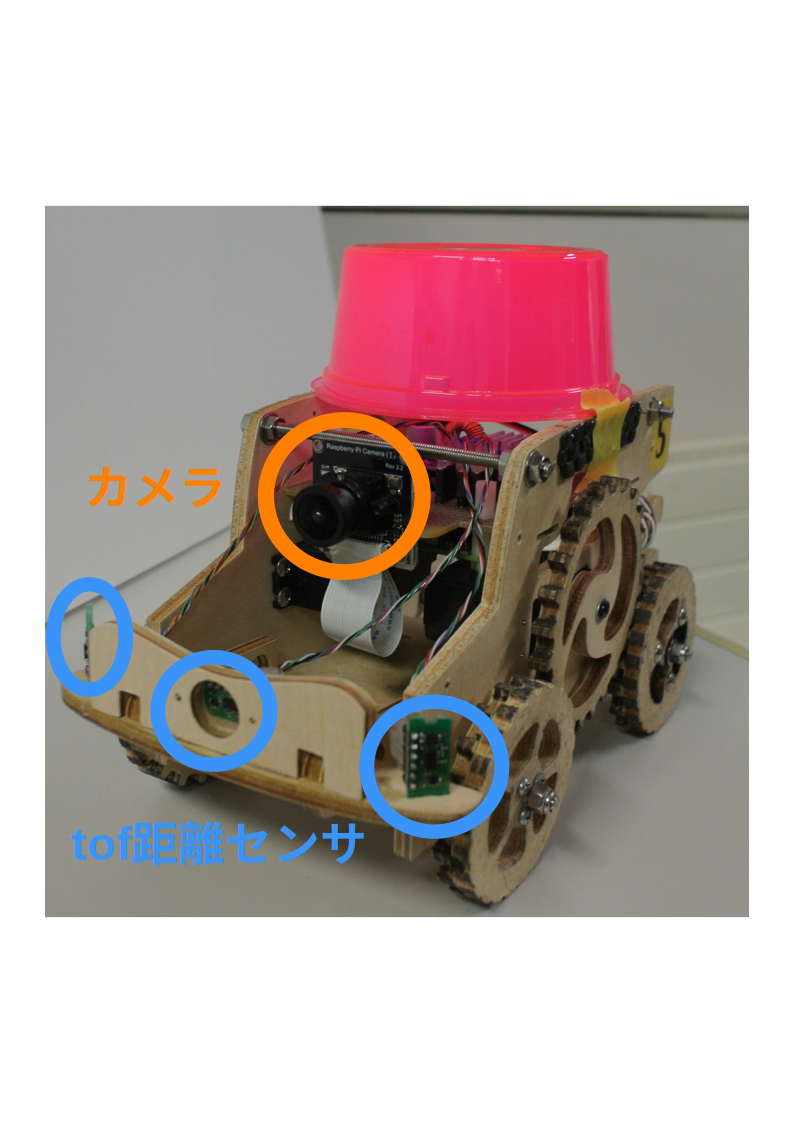
\includegraphics[height=7cm,width=0.8\linewidth]{pic/robo.png}
  \vspace{-10mm}
  \caption{使用する走行ロボット}
  \label{fig:ssr2}
\end{center}
\end{figure}
%先行研究では2輪駆動の走行ロボット(図\ref{fig:old_2dovr})で実験を行っていた.
\vspace{-3.5mm}
\subsection{他機体認識}
本研究では複数の走行ロボットの集団行動を観測する.
そのため,ロボットは自身とは別の機体の相対角度と位置を認識しなければならない.
他機体認識に使用するセンサはRaspberry Pi Cameraである.
本研究ではこのカメラを用いてロボット上部に取り付けられたピンク色のカップから他機体との相対角度と距離を認識している.
距離を求める際に,カメラに写ったピンク色のカップの幅から最小二乗法を用いてフィッティングを行った.
\vspace{-1.5mm}
\subsection{相乗平均距離と疑似的弾性散乱}
本研究では,弾性境界を考慮する必要性があるため,ロボットは壁や他機体を検出して反射する必要がある.
そのためにtof距離センサを用いる.
壁や他機体に近づいた際には,弾性散乱を行うために3つ装着されているtof距離センサから得られる距離データの相乗平均を(\ref{areaL})式,(\ref{areaR})式で求める.
ここで$ \gamma = 0.33 $とし,3つのtof距離センサから得られる距離データを等加重で計算を行う.
相乗平均距離を使用する理由としては,障害物に近づいた際に,より反応しやすくするために用いる.

$d_{C} $は中央の距離センサの距離データ,$d_{L} $は左の距離センサの距離データ,$d_{R} $は右の距離センサの距離データである.tof距離センサから得られる距離データの単位は[m]である.
\begin{eqnarray}
\label{areaL}
\bar{d_{L}} = d_{C}^{\gamma} \times d_{L}^{1 - \gamma} \\
\bar{d_{R}} = d_{C}^{\gamma} \times d_{R}^{1 - \gamma}
\label{areaR}
\end{eqnarray}
本研究では,$\bar{d_{L}}$ または$\bar{d_{R}}$が$0.2$以下になった場合はその場で$\bar{d_{L}}$と$\bar{d_{R}}$の値が大きい方へ$0.3$秒間,出力$100\%$で方向転換する.
方向転換を擬似的弾性散乱とみなす.
\vspace{-1.8mm}
\section{走行実験}
本研究では,図\ref{fig:cource}のようなドーナツ型コースを用いて走行実験を行う.
外側の壁は半径2[m]の円,内側の壁は半径1[m]の円である.
初期状態として,コースに8台のロボットを4台は時計回りに配置,残りの4台は半時計回りに配置して実験を行う.
\begin{figure}[ht]
\begin{center}
  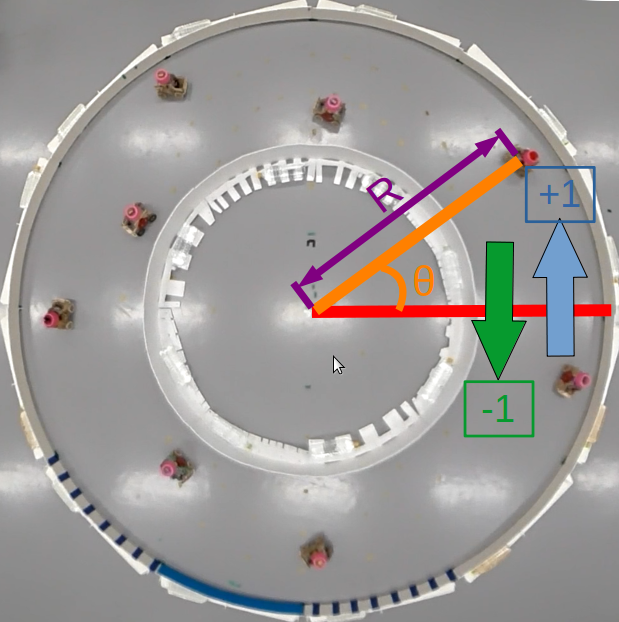
\includegraphics[height=4.9cm,width=0.7\linewidth]{pic/cource3.png}
  \caption{実験コース}
  \label{fig:cource}
\end{center}
\end{figure}
走行実験では,2種類のアルゴリズムで走行させ,流量を比較する.
1つ目のアルゴリズムは,弾性散乱のみで走行するアルゴリズムである.
$\bar{d_{L}} < 0.2$もしくは$\bar{d_{R}} < 0.2$であれば,弾性散乱を行う.
それ以外の場合には進行方向正面に進むアルゴリズムである.

2つ目のアルゴリズムは,2次元最適速度旋回アルゴリズムで走行するアルゴリズムである.
他機体を発見した場合は近づいていき,それ以外の場合は進行方向正面に進み,相乗平均距離で弾性散乱も行う.
パラメータは$a=3.0$[1/s], $\alpha=0.15$[m/s], $\beta=8.0$[1/m], $b=0.3$[m], $c=1.0$で実験を行う.
\vspace{-2.5mm}
\subsection{評価方法}
走行実験は流量という観測量を用いて定量的に評価する.
流量の計算式は式(\ref{func:flowrate})である.パラメータは$l$:全走行ロボットの通過回数,$t$[min]:計測時間,$w$[m]:使用したコースの道幅である.
%表\ref{table:flow}に示す.
\vspace{-2.0mm}
\begin{eqnarray}
f_{rate} = \frac{l}{tw}
\label{func:flowrate}
\end{eqnarray}
実験コース(図\ref{fig:cource})の右側にある赤色の直線を基準線とする.
その基準線を時計回り(緑矢印の向き)に通過すると通過回数を$-1$回,反時計回り(水色矢印の向き)に通過すると通過回数を$+1$回する.
\vspace{-2mm}
\section{実験結果}
弾性散乱のみでの走行と2次元最適速度旋回アルゴリズムでの走行を行った.
走行状態を表すグラフを図\ref{fig:theta_2dovr}$\sim$図\ref{fig:R_ela}に示す.

図\ref{fig:theta_2dovr},図\ref{fig:theta_ela}のグラフは走行ロボットの$\theta$と時間の関係図である.
横軸は時間[秒],縦軸は角度$\theta$[rad]である.図\ref{fig:R_2dovr},図\ref{fig:R_ela}のグラフは走行ロボットの時間変化におけるコース中心からの直線距離を表している.

図\ref{fig:theta_2dovr}のグラフに注目し,実験開始から約80秒までは$\theta$のグラフが途中で折れ曲がっている.これはロボットが方向転換している状態である.
約80秒以降は$\theta$の変化が一定であることから,このロボットは時計回りに走行している.

%約80秒までは,$\theta$が増加・減少を繰り返している.
%これは,ロボット同士が対面走行している状態である.
%約80秒以降だと,走行ロボットは方向転換を行わず,一方向走行になっている.
%ひも状走行が形成された場合には,図\ref{fig:R_2dovr}の約80秒以降のようなグラフとなる.

弾性散乱のみで走行した場合のグラフである図(\ref{fig:theta_ela})を見ると,実験終了まで$\theta$のグラフが折れ曲がっている.
2次元最適速度旋回アルゴリズムでの走行に比べると不安定な走行状態である.

時間変化における$\theta$のグラフから,2次元最適速度旋回アルゴリズムでは,約80秒以降で時計回りに走行している.
図\ref{fig:R_2dovr}をみると,実験開始から約80秒まではコース内を約60cm移動していることが読み取れる.
これは,対面走行時に他のロボットと衝突しないよう回避行動をとっているため,Rの値が大きく変動している.
約80秒以降だと,Rの変化が減少傾向にあることから,他のロボットを回避する行動が少ない走行状態だと言える.

弾性散乱のみで走行した場合には2次元最適速度旋回アルゴリズムと比べて,実験終了時までRの値が大きく変動している.
これは全ロボットが一方向で走行しているのではなく,対面走行状態になっている可能性が高いと言える.
本研究で使用するコースは図\ref{fig:cource}の円形コースであり,比較的密度が低いことから,対面走行,一方向走行時であっても,ロボットはコースの内側や外側に寄る.
このように,$\theta$とRのグラフ両方から,走行ロボットの走行状態を予測することが可能である.
\begin{comment}
走行状態を観察すると,弾性散乱のみのアルゴリズムだと,8台全てが一方向走行を形成する場面が存在する.
しかし他機体を追従するアルゴリズムは組み込まれていないため,一方向走行が安定しているとは言えない.
一方で2次元最適速度旋回アルゴリズムでは,一方向走行が形成された場合には安定して一方向走行になる.
対面同士で接近した場合にはお互い正面から向かって行くので,一方向走行が形成されるのに時間がかかる.
\end{comment}
%\vspace{-20mm}
\begin{figure}[h]
\begin{center}
  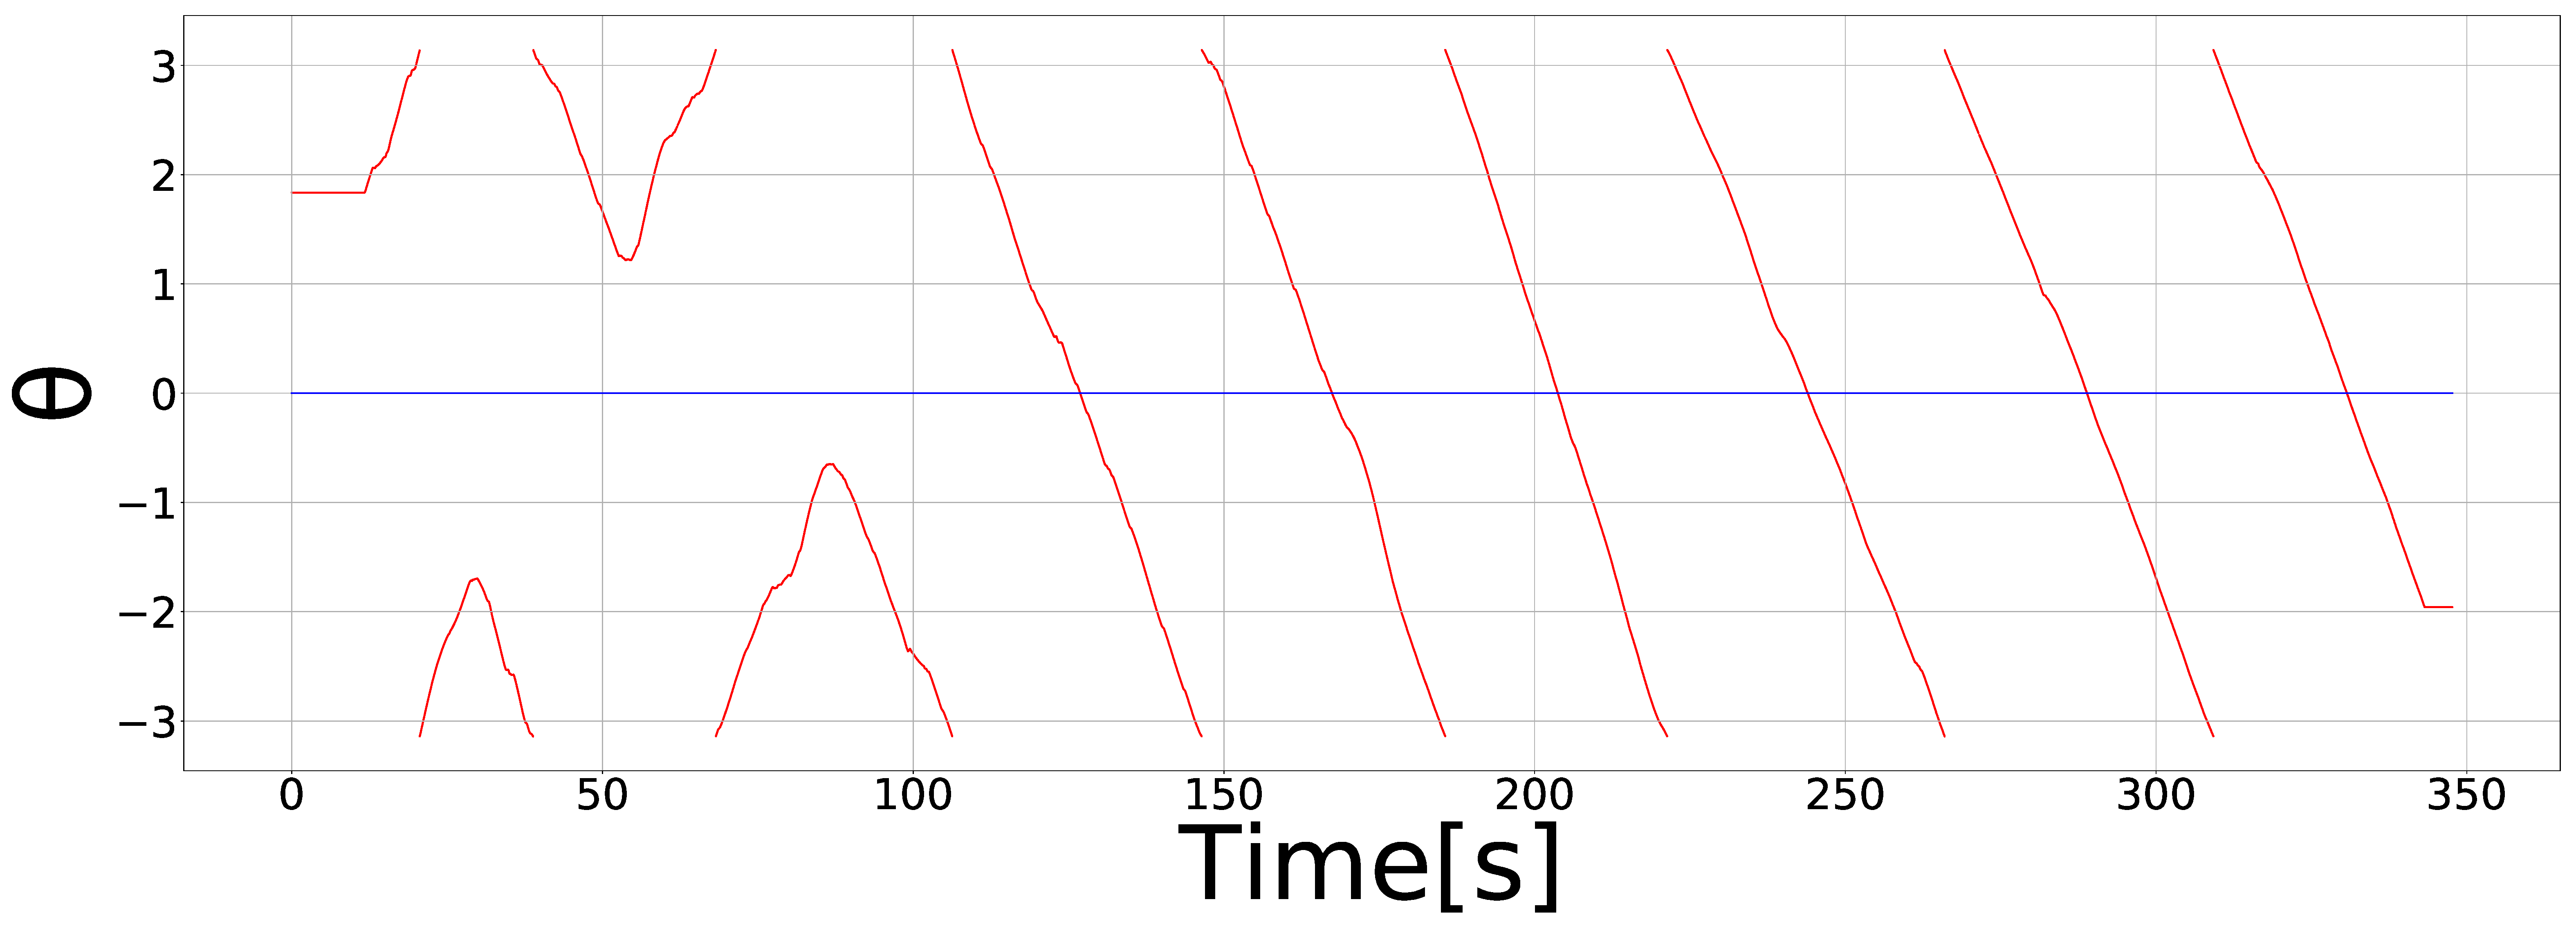
\includegraphics[width=0.85\linewidth]{pic/106_shita.eps}
  \vspace{-3mm}
  \caption{走行中の時間変化における角度変化(2dovr)}
  \label{fig:theta_2dovr}
  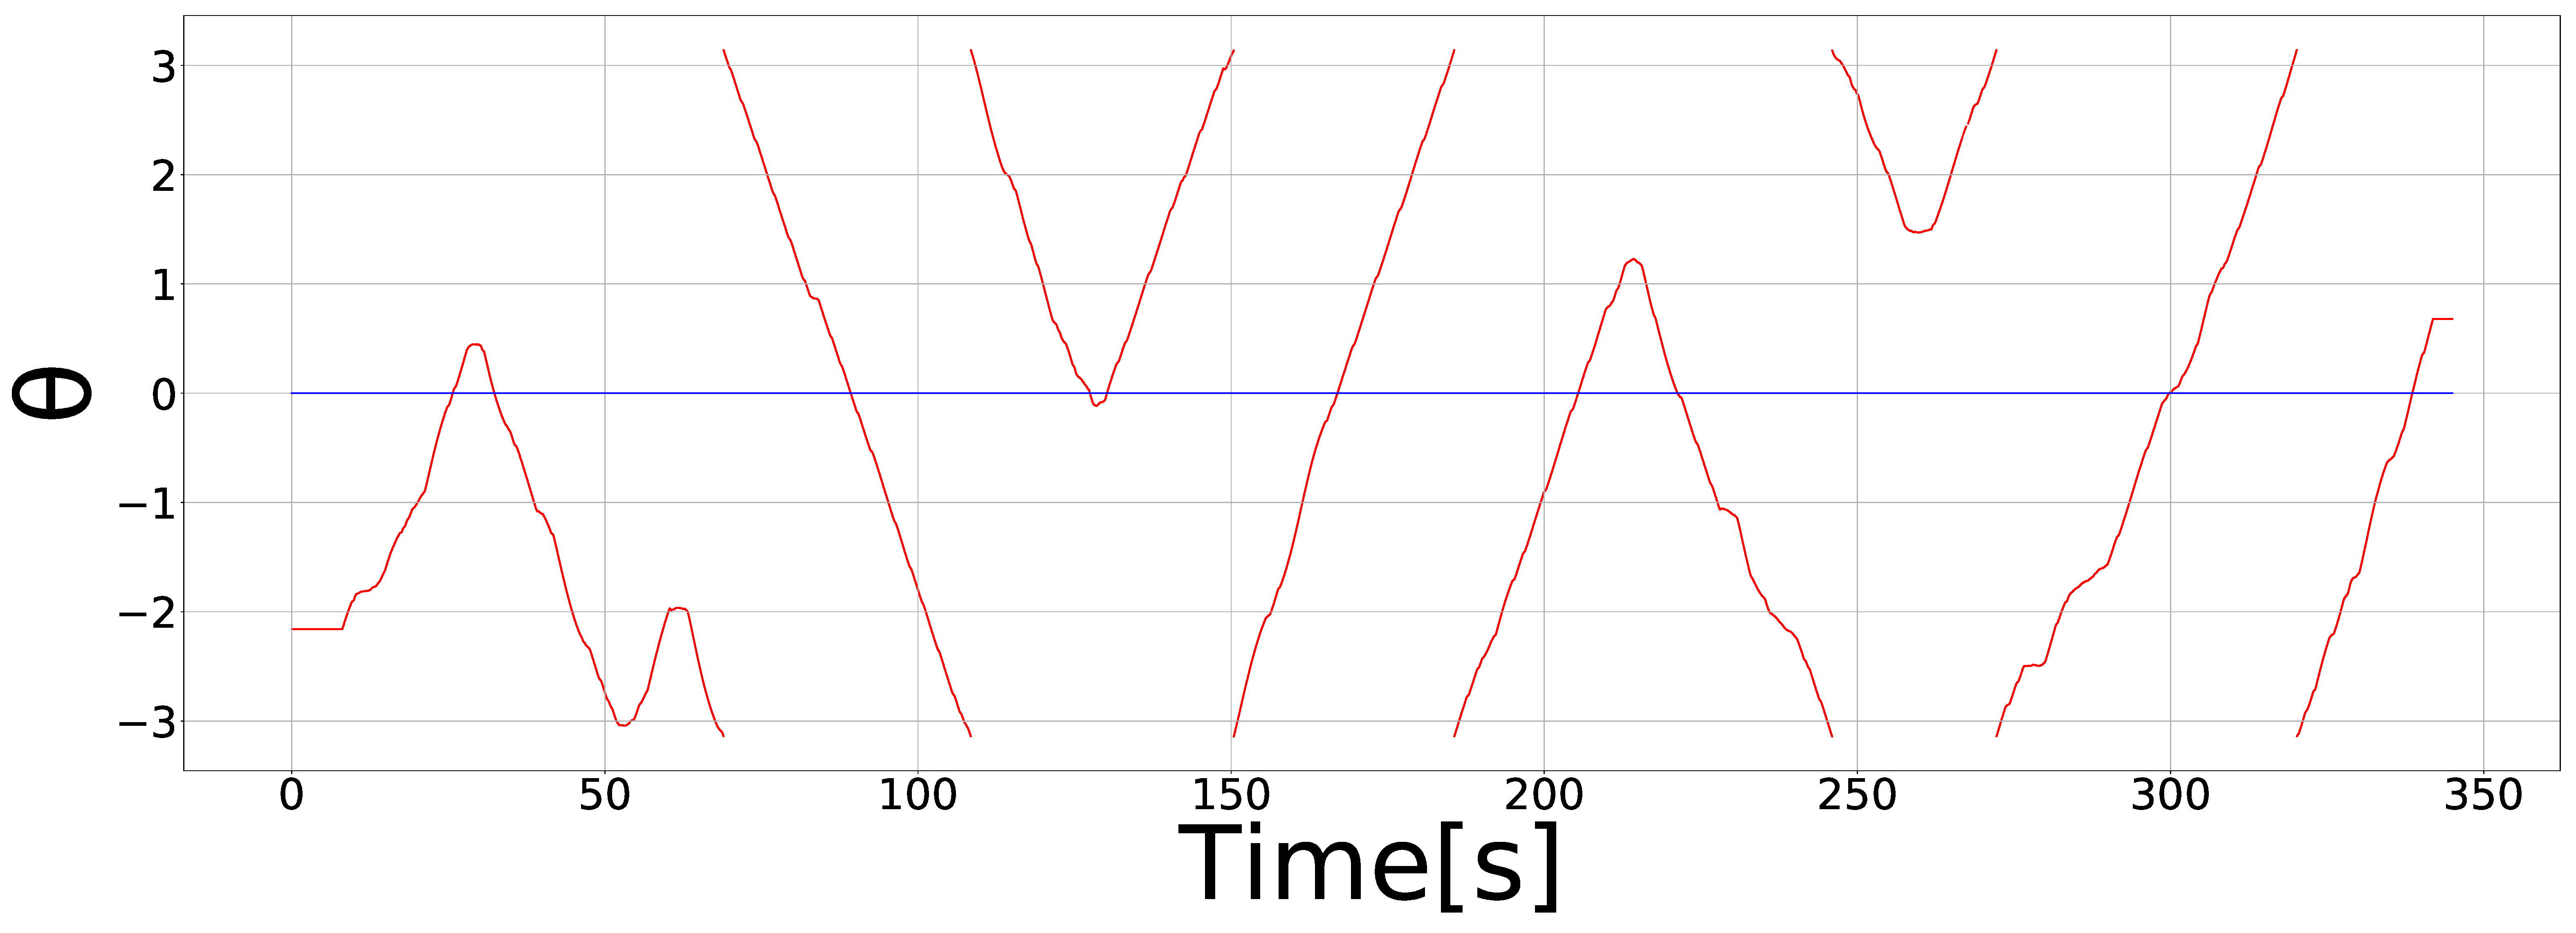
\includegraphics[width=0.85\linewidth]{pic/112_shita.eps}
  \vspace{-3mm}
  \caption{走行中の時間変化における角度変化(弾性散乱)}
  \label{fig:theta_ela}
  %\vspace{-2mm}
  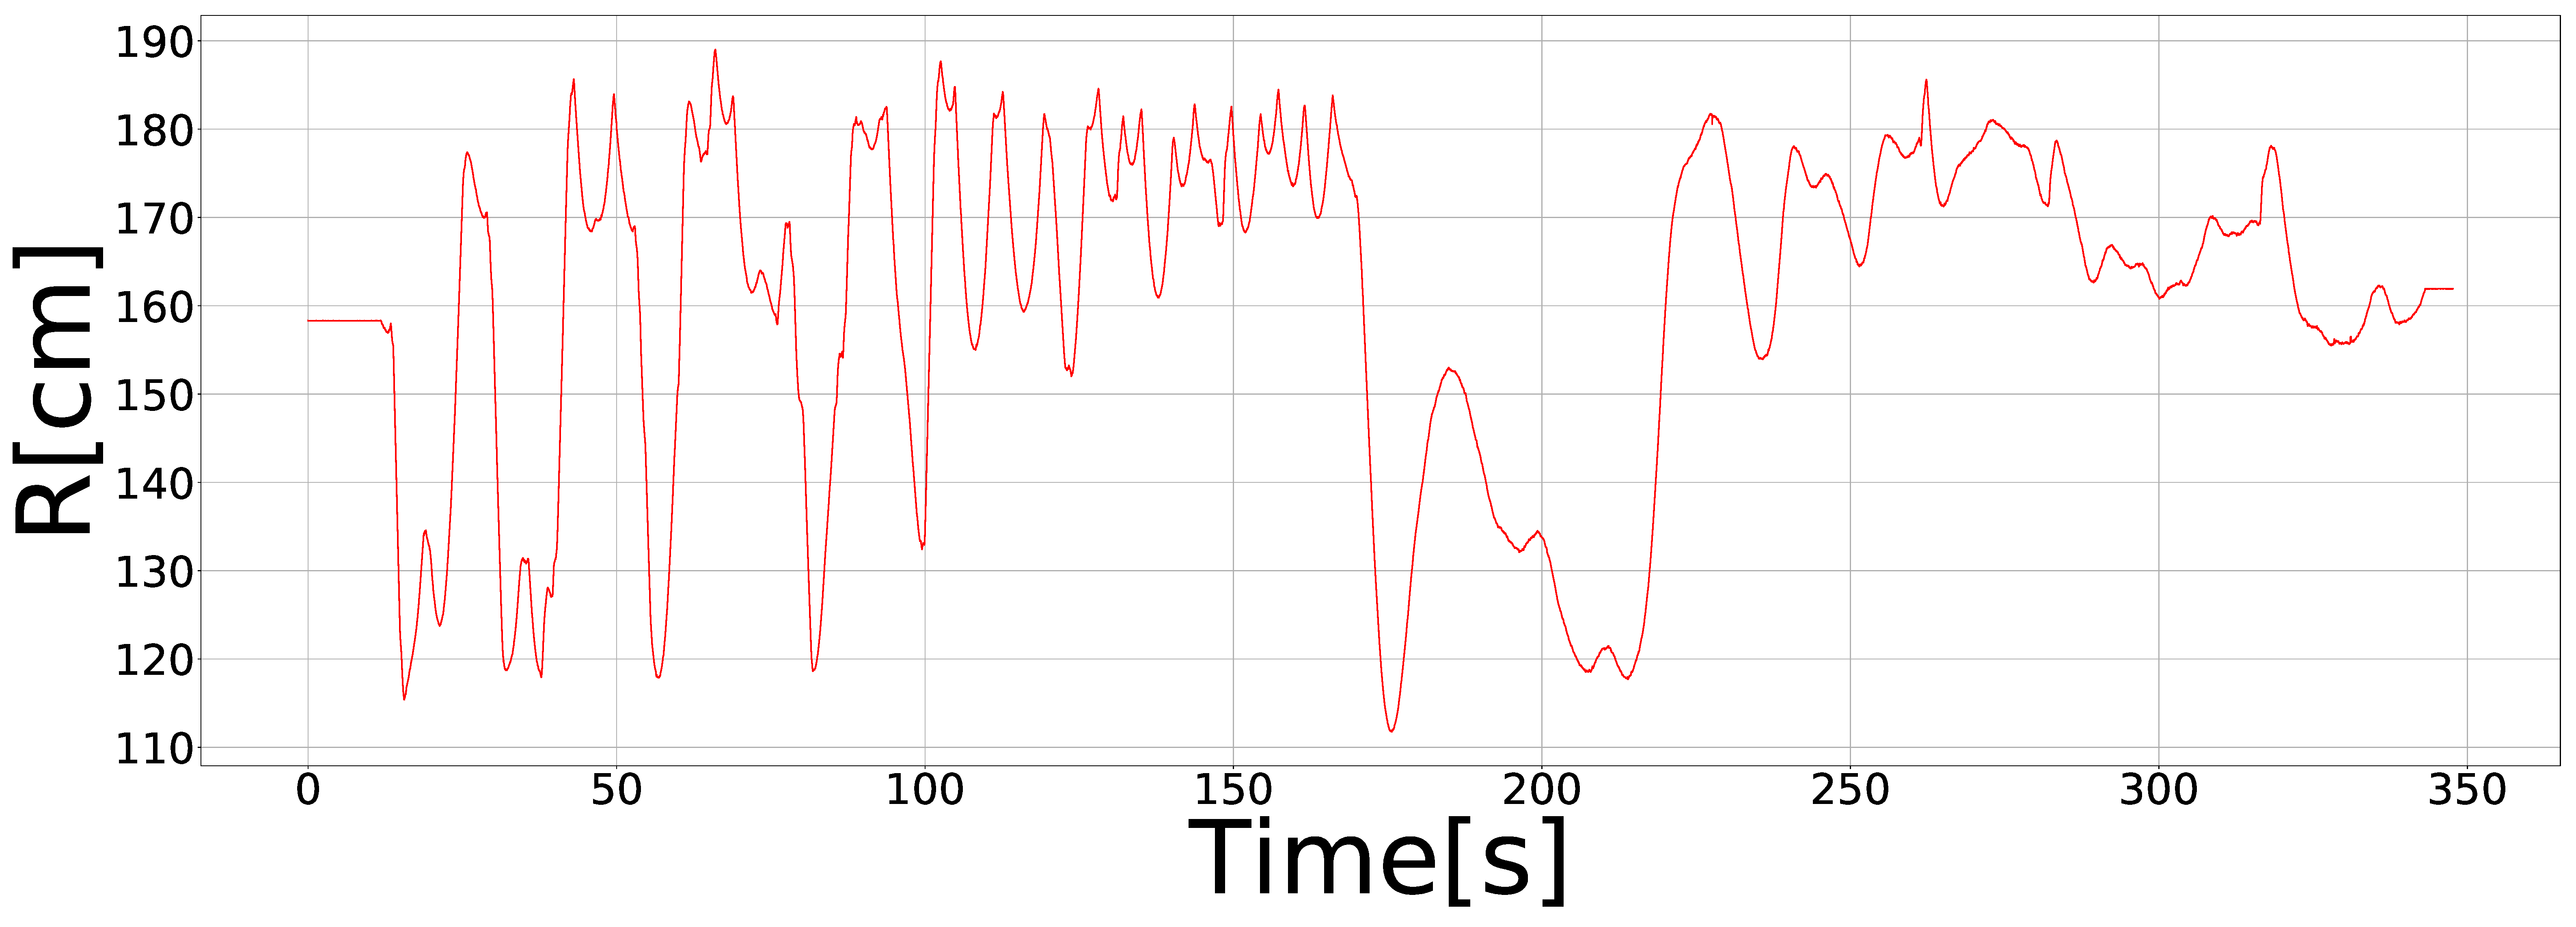
\includegraphics[width=0.85\linewidth]{pic/106_R.eps}
  \vspace{-3mm}
  \caption{走行中の時間変化における半径の変化(2dovr)}
  \label{fig:R_2dovr}
  %\vspace{-2mm}
  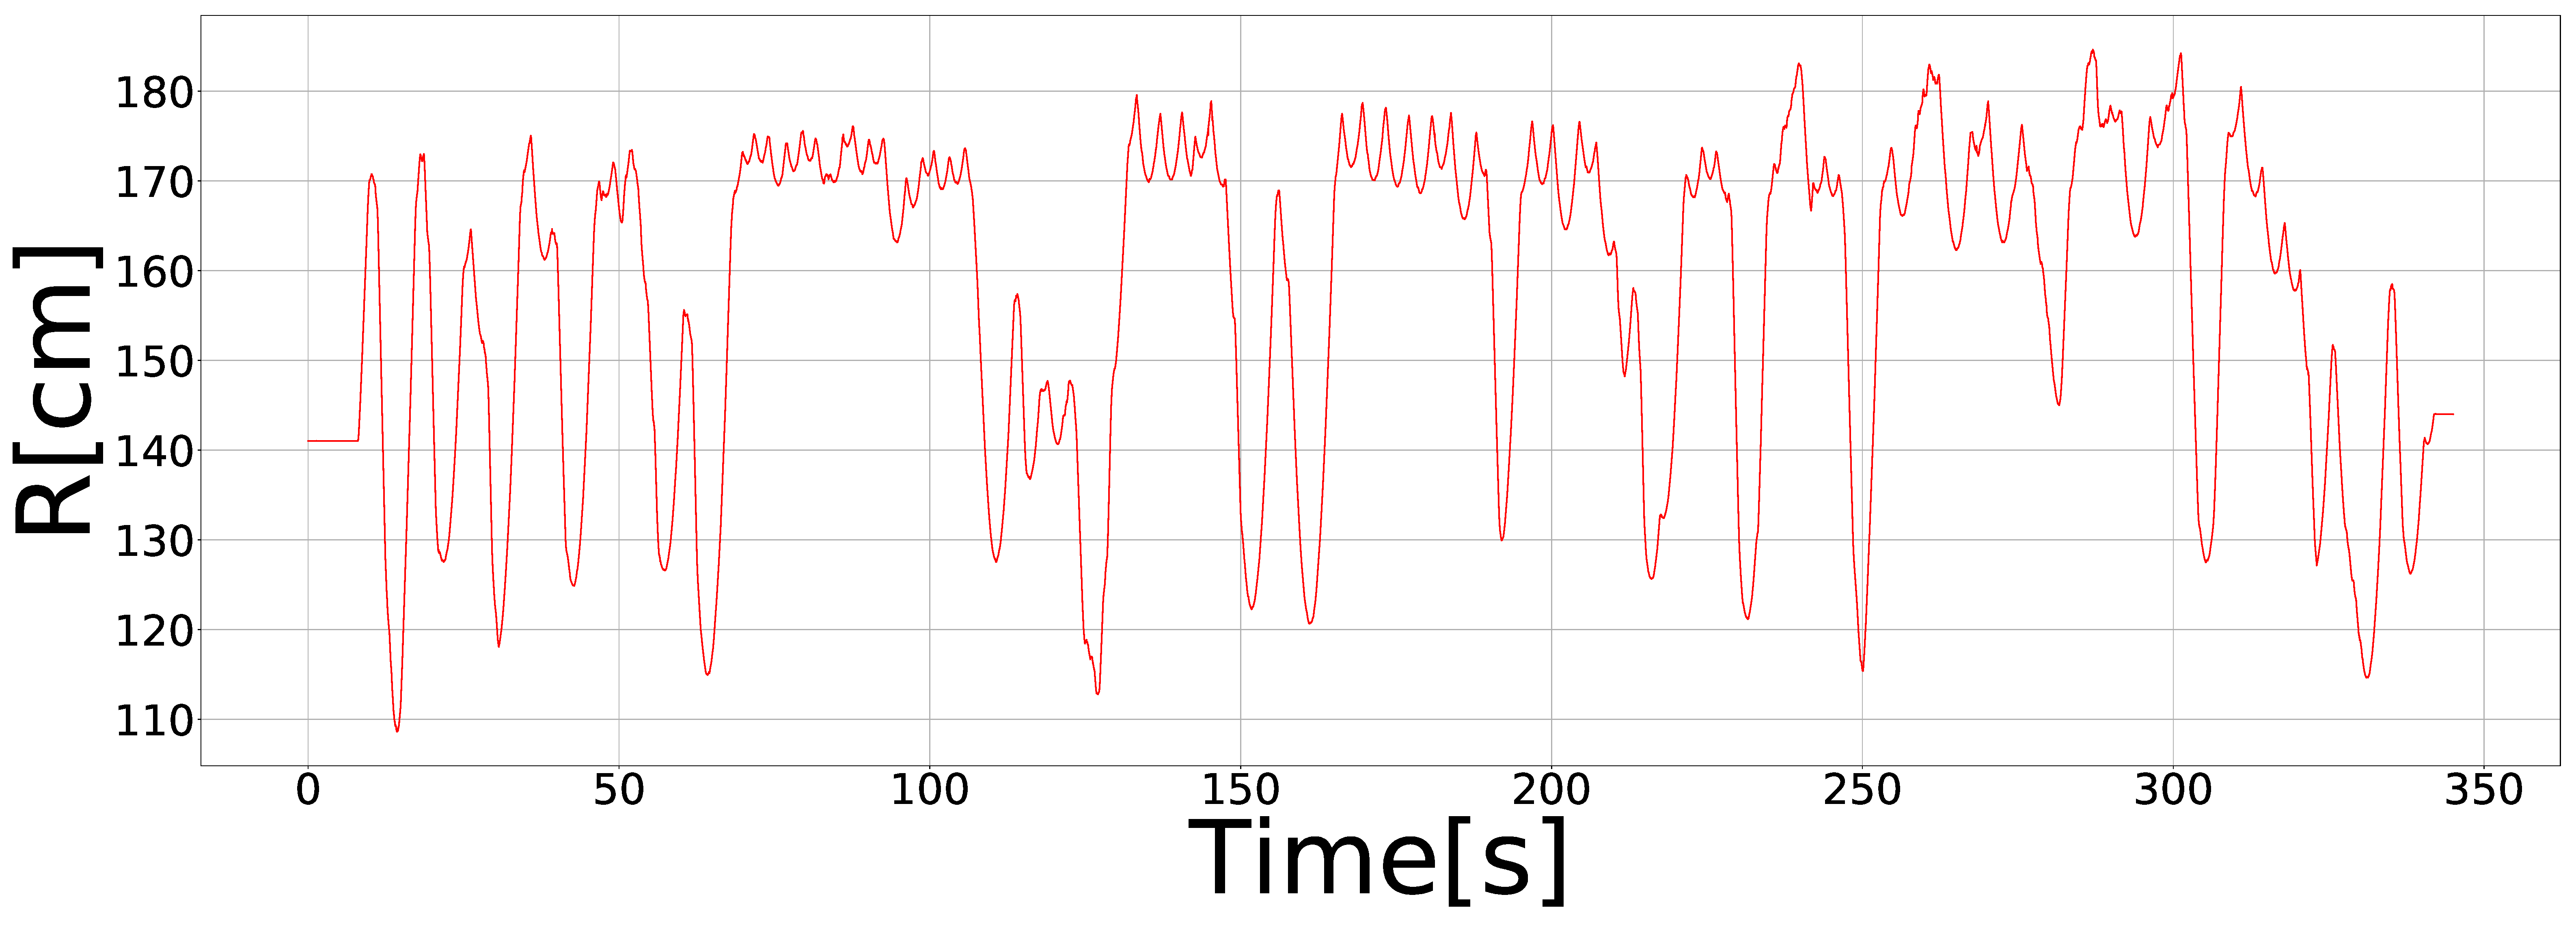
\includegraphics[width=0.85\linewidth]{pic/112_R.eps}
  \vspace{-3mm}
  \caption{走行中の時間変化における半径の変化(弾性散乱)}
  \label{fig:R_ela}
  %\vspace{-2mm}
\end{center}
\end{figure}

\begin{comment}
8台走行の流量を比較する基準として,コース内をロボット1台で走行した流量を基準として用いる.
2種類のアルゴリズムで走行した場合の流量は弾性散乱,2次元最適速度旋回アルゴリズム共に$2.0$となった.
この値を基準として複数台走行時の流量と比較する.各7回実験の単位時間あたりの流量のグラフは図\ref{fig:flowrate}である.

弾性散乱で走行するアルゴリズムでは,流量の変動が大きい.
図\ref{fig:flowrate}内の緑色の横線が1台で走行した際の流量であり,1台のみでの走行の流量を下回っている実験結果もある.
2次元最適速度旋回アルゴリズムは弾性散乱のみの走行と比較すると,変動は小さい.

各7回の実験結果を平均すると,弾性散乱で走行した際の平均流量は$6.1$,2次元最適速度旋回アルゴリズムで走行した際の平均流量は$7.4$となった.
わずかに2次元最適速度旋回アルゴリズムで走行したほうが流量が増える結果である.
\end{comment}
合計7回の走行実験のの平均流量は,弾性散乱のみで走行した場合は$6.1$,2次元最適速度旋回アルゴリズムで走行した場合は$7.4$となった.

\vspace{-3mm}
\section{まとめと今後の課題}
本研究は先行研究との相違点として,センサとカメラの画角を変更した.また新たに,2次元最適速度旋回アルゴリズムを開発した.
外側の壁は半径2[m],内側の壁は半径1[m]のコース幅1[m]の円形フィールドで走行ロボット8台を用いて走行実験を行った.
2種類のアルゴリズム(2次元最適速度旋回アルゴリズム,弾性散乱のみを行うアルゴリズム)で走行させ,流量という観測量で比較を行った.
結果として,2次元最適速度旋回アルゴリズムの方が流量が増えるという結果になった.本研究で扱う2次元最適速度旋回アルゴリズムのパラメータは種類が多く,他のパラメータを使用し実験を行っていきたい.
\vspace{-3mm}
\begin{thebibliography}{99}
\bibitem{mygm} 川野多佳也,宮島高志,本田泰,二次元最適速度ロボットの開発と集団走行実験,第23回交通流と自己駆動粒子系のシンポジウム論文集,p63-p66,(2018)
\bibitem{ov2} 石渡龍輔,衣川亮太,杉山雄規,Kantorovicmetricを用いた2次元OV粒子の集団流の感応度依存性の解析,第22回交通流と自己駆動粒子系シンポジウム論文集,P41-44,(2016)
\end{thebibliography}
\end{document}


